\chapter{In Progress and Upcoming}
\section{Experiment 3: DenseCap}
The task on which a feature extractor is trained will affect the type of features it learns to identify. The goal of this experiment is to see if a model originally trained on a more language based task, such as captioning, identifies more relevant features for answering the questions than one trained on visual tasks. \\ % SD 2021-05-01 16:19:41 +0200: Dense-cap provides both visual and linguistic common sense knowledge to us. It identifies objects, identifies them with their names and then describes their relations. Hence, we believe that this will help question answering as the information which will be much richer both in terms of vision and language from what the model has experienced out in the wild before from internal CNN training. DenseCap was trained on a variety of images and objects and descriptions inform us how humans structure and see the world.
The DenseCap model performs the 'dense captioning' task, in which the model identifies areas of interest in the image, and then provides a caption for each area\cite{densecap}. An example of the DenseCap output for an image from the scene dataset can be seen in Fig.~\ref{fig:example_densecap}. Some of the captions are a little bit weird, such as 'bathroom with walls and walls', but the model is identifying aspects such as color and material, which would be helpful in answering the types of questions being asked in the VQA portion. 

% SD 2021-05-01 16:30:49 +0200: Explain how we are going to use DensceCap features as here there are various options. For example, we will extract n bounding boxes and extract their visual features and concatenate them in a large vector. Or we could also take labels of these objects and hope that language will help. Another possible variant would be to test the internal CNN features for the image and then add object extracted features with DenseCap as just described: this way we have an overall scene representation (hopefully asccurate since internal CNN would be good at internal scenes) and have object information from external CNN.

\begin{figure}[h]
     \centering
     % \includegraphics[width=.5\textwidth]{/home/yasmeen/Desktop/thesisproj/thesis/figure/example_densecap.png}
     \includegraphics[width=.5\textwidth]{./figure/example_densecap.png}
     \caption{DenseCap output for image from dataset}
     \label{fig:example_densecap}
\end{figure}

% SD 2021-05-01 16:33:21 +0200: Why are we adding DenseCap features also **after** the attention layer?


\subsection{Using DenseCap Features}
The first task, which is currently in progress, is to completely replace the original EQA CNN and use DenseCap as the feature extractor, as shown in Fig.~\ref{fig:densecap_feats}.

\begin{figure}[h]
     \centering
     % \includegraphics[width=.5\textwidth]{/home/yasmeen/Desktop/thesisproj/thesis/figure/densecapsketch.png}
     \includegraphics[width=.5\textwidth]{./figure/densecapsketch.png}
     \caption{Model With Densecap}
     \label{fig:densecap_feats}
\end{figure}


\subsection{Using DenseCap Boxes}
Since DenseCap identifies areas of interest, these boxes can be used to give the model information about where objects are. I plan to give the model these boxes, along with the top-down features of the entire scene, as shown in Fig.~\ref{fig:densecap_boxes}. 

% SD 2021-05-01 16:35:55 +0200: The boxes are the visual features per each object. The feats are the top-down (if we use Andersson, or bottom-up if we use our terminology) features of the entire scene. It is here where we could either use pre-trained or internal CNN visual features.

\begin{figure}[h]
     \centering
     % \includegraphics[width=.5\textwidth]{/home/yasmeen/Desktop/thesisproj/thesis/figure/densecapboxes.png}
     \includegraphics[width=.5\textwidth]{./figure/densecapboxes.png}
     \caption{Model With Densecap Boxes}
     \label{fig:densecap_boxes}
\end{figure}

\section{Experiment 4: Look Around}
The previous experiments focus on giving more sources of information to the model. The planned 'Look Around' experiment would attempt to improve the information being given instead. The VQA model takes in the last five frames of navigation as its visual input. However, as seen in Fig.~\ref{fig:example_vqa_result}, these images are very similar to each other, and with odd angles of the object in consideration. The plan for this experiment is to implement a look around procedure, where the agent makes a series of moves (look left, look right, etc) at the end of navigation, so that the last five frames will give more varied viewpoints of the room and object, and these frames will be used as the visual input to VQA.

% SD 2021-05-01 16:38:46 +0200: From the look-around samples we will have to determine what are releavnt things in the scene. Run densecap on several images that we sample through look around. Identify salience of features/objects; hence make some more relevant and some less relevant. Bias QA by looking at the relevant features and discard the less relevant features. This way we could also get in into the question of attention.

\section{Experiment 5: Visual-Linguistic BERT}
The last experiment I hope to conduct is to compare the previous model with a state of the art model using a transformer. VL-BERT is pretrained for visual linguistic tasks, using a combination of captioning and text-only tasks\cite{VLBERT}. VL-BERT performed well on the standard VQA task, so it makes a good comparison for a model designed specifically for this task. 

% NI 2021-05-17: how exactly are you planning to use these models? as encoders? LX-MERT can be a better option to use here (because of pre-training tasks and higher modularity): https://arxiv.org/pdf/1908.07490.pdf
% NI 2021-05-17: another good paper: https://arxiv.org/pdf/2104.12763.pdf

